\section*{Conclusione}

Possiamo dire che abbiamo compreso come funziona un oscillatore a ponte di Wien e le problematiche ad esso associate. In particolare vogliamo riportare un grafico, Fiura \ref{fig:instabilita} dell'andamento della tensione di output $V\ped{out}$  dell'oscillatore nelmomento in cui abbiamo applicato dei condensatori di disaccoppiamento sull’alimentazione dell’amplificatore operazionale.
Come si può osservare l'uscita diventa instabile, tuttavia non siamo in grado di dare una spiegazione del perchè succeda tale fenomeno. 

\begin{figure}[h]
    \centering
    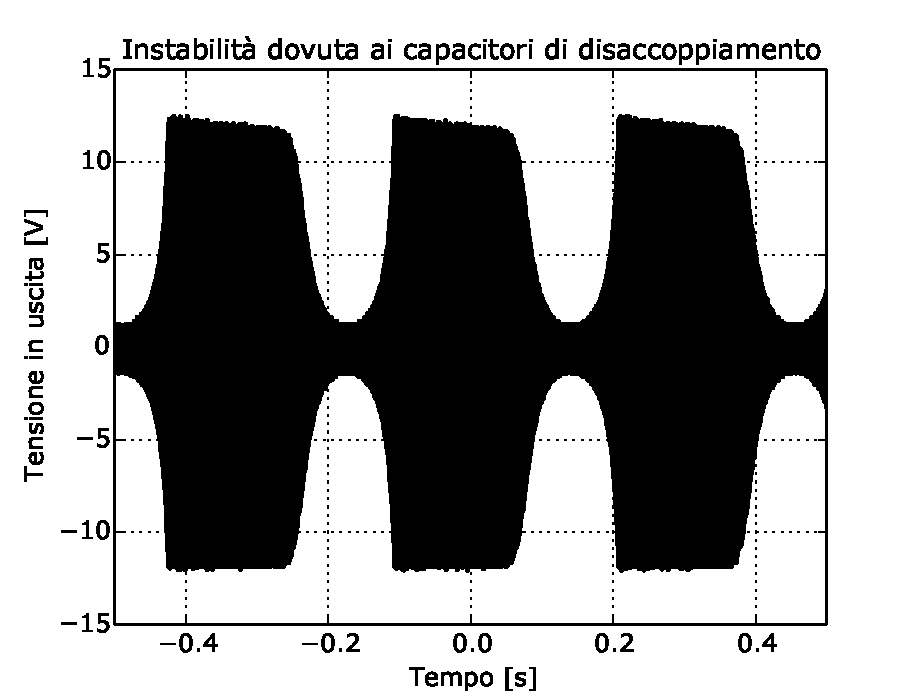
\includegraphics[width=0.7\columnwidth]{figure/inststab.pdf}
    \caption{Questo grafico mostra la ensione in uscita dall'oscilloscopio ne caso in cui siano presenti delle capacità di disaccoppiamento sulle almentazioni dell'amplificatore operazionale. Possiamo commentare che l'intervallo tra un picco ed una altro del segnale in uscita è dell'ordine dei \SI{0.3}{\second}}
    \label{fig:instabilita}
\end{figure}